\documentclass[11pt]{article}

% ============================================================================
% Paper 5 -- Even synthesis is transport. arXiv / Zenodo preprint source.
% Compile: pdflatex x2.
% ============================================================================
\usepackage[utf8]{inputenc}
\usepackage[T1]{fontenc}
\usepackage{amsmath,amssymb}
\usepackage{graphicx}
\usepackage{booktabs}
\usepackage{geometry}
\usepackage{xcolor}
\usepackage[hidelinks]{hyperref}
\usepackage{caption}
\usepackage{enumitem}
\usepackage{authblk}

\geometry{a4paper, margin=1in}
\captionsetup{font=small, labelfont=bf}
\setlist{nosep, leftmargin=1.4em}

\title{\bfseries Even Synthesis Is Transport:\\
At 3B, Implicit Multi-Hop Reasoning Reduces to Retrieval-and-Elimination,\\
and Composition Appears Only as Externalized Self-Delivery}

\author[1]{Evgenii Vyaltsev\thanks{ORCID 0009-0004-3712-6798. Correspondence: handle \texttt{@seqe\_phi}.}}
\author[1]{Daniil Vyaltsev}
\affil[1]{Independent Researcher}
\date{June 2026}

\begin{document}
\maketitle

\begin{abstract}
\noindent
Retrieval can be explained as transport: a prior program showed that long-context
retrieval failure is repaired by \emph{delivering} a fact, not by redirecting
attention or by a reusable internal correction. Synthesis is where that account
should break: in an $A\!\to\!B\!\to\!C\!\to\!D$ chain the target $D$ is \emph{absent}
from context and must be \emph{assembled}, so a model that only transports cannot
answer --- unless it composes. We test, pre-registered and cross-model
(Llama-3.2-3B, Qwen2.5-3B; greedy; both vanilla bases), \emph{when} $D$ forms
(prefill vs.\ decode) and \emph{whether the stated hops are used}, with four locked
controls and a built-in positive control. The verdict replicates on both models.
\textbf{Implicit (no scratchpad --- the clean computation test): reduces to delivery.}
Three independent operationalizations agree: (i) in-place \emph{corruption} of the
middle hop flips the answer in only $5\%$/$11\%$ of cases the model gets right, while
corrupting the code fact flips $100\%$; (ii) masking the link facts at the
answer-emitting step is inert, masking the code kills it; (iii) blocking the
elimination shortcut with decoys floors implicit accuracy to chance
($0.35\!\to\!0.07$, $0.45\!\to\!0.10$). The model answers by
\emph{retrieval-and-elimination} over competitor facts, not by traversing the stated
edges. \textbf{Explicit chain-of-thought: genuine traversal --- but scaffolded by
self-delivery.} Writing the trace makes every hop causal and corruption disrupts the
answer ($84\%$/$90\%$ middle-hop flip --- the positive control proving the implicit
null is a real null, not a broken test), and it is decoy-robust; but the model
composes by writing each intermediate fact \emph{into} context and reading it back ---
converting computation into delivery (self-RAG), not internal decode-time binding.
We also surface a methodological catch: under competition, node \emph{removal} is
confounded by elimination (a removed mid-fact is recoverable from competitors), so
removal under-states hop usage; in-place \emph{corruption} is the faithful test.
Conclusion, regime-bounded: at $3$B, internal multi-hop computation of an absent fact
does not occur; ``reasoning'' here is retrieval-and-elimination, and real composition
appears only as externalized self-delivery. This closes the synthesis regime in the
same direction as attention ($\gamma$: transport) and the delivery ladder
(repair $=$ deliver the binding): in this model class the network \emph{delivers and
composes through an external buffer; it does not latently compute}. The null is the
strongest of the three, because synthesis is the one place transport could have
failed --- and it did not. Code, pre-registration, and raw per-case logs are released.
\end{abstract}

\section{Introduction}
\label{sec:intro}

Two prior results in this program localize the mechanism of long-context behaviour to
\emph{transport}. Up-weighting a needed key's attention buys nothing beyond plain
re-delivery, so attention is weighted transport, not
computation~\cite{paper3retention}; and the repair for retrieval-disambiguation
failure is delivering the attribute$\to$code \emph{binding} --- not attention
redirection and not a transplanted state correction, both of which are
closed~\cite{paper4arc}. Each was a retrieval task: the answer is \emph{present} in
context, and the question is whether the model moves it to the output.

Synthesis is the adversarial case for that account. In a composed chain
$A\!\to\!B\!\to\!C\!\to\!D$ where $D$ is bound only to $C$ and the question names only
$A$, the answer $D$ is \emph{not present anywhere}; it can only be produced by
chaining the hops. A pure transporter has nothing to transport. If the program's
``everything is transport'' reading is going to fail, it should fail here. We
therefore make synthesis the decisive test, and we sharpen the question from ``does
synthesis happen'' to \emph{when does the target form and are the stated hops used}:
\begin{itemize}
\item \textbf{P1 decode-computation:} the binding $A{+}B{+}C\!\to\!D$ happens at the
answer step --- the positive mechanism we would hope to find.
\item \textbf{P2 prefill-assembly:} $D$ is already encoded during reading; decode
merely emits it --- still transport, of a representation formed at read-time.
\item \textbf{P3 reduces-to-delivery:} the ``chain'' is not traversed --- a single
code fact plus elimination over competitors solves it --- retrieval in disguise.
\end{itemize}
We pre-register four controls to separate these (necessity of each node; a
false-hop usage test; mask-at-answer for prefill-vs-decode; a decoy sweep that blocks
elimination), run both ported 3B models, and report implicit and chain-of-thought
separately because explicit CoT writes intermediate facts into context and thereby
\emph{is} a form of delivery. The result, replicated on both models, is P3 for
implicit and self-delivered traversal for CoT.

\paragraph{Relation to the program.}
This is the capstone of a three-gate arc: $\gamma$ (attention $=$ transport,
\cite{paper3retention}), the delivery ladder (repair $=$ delivery,
\cite{paper4arc}), and synthesis (here). The first two concern retrieval; this paper
contributes the synthesis gate and the cross-arc thesis. The unifying claim ---
\emph{this model class delivers and composes via an external buffer but does not
latently compute} --- now rests on three independent causal gates, cross-model.

\section{Related work}
\label{sec:related}

\textbf{Multi-hop reasoning and latent composition.} Whether transformers compose
facts internally or rely on shortcuts is actively debated; work on latent multi-hop
reasoning finds it weak and entity-dependent~\cite{yang2024latent}, and the ``grokked
transformers'' line shows implicit composition emerging only under heavy
training~\cite{wang2024grokking}. Our contribution is a \emph{causal} usage test
(corruption, mask-at-answer) on off-the-shelf 3B models, with a decoy control that
isolates an elimination shortcut. \textbf{Chain-of-thought as externalization.} CoT
improves multi-step accuracy~\cite{wei2022cot}; analyses question whether the written
trace is faithful to the computation~\cite{lanham2023faithfulness}. We give a
mechanistic reading: in this regime CoT \emph{is} the mechanism --- the model composes
by writing and re-reading, self-delivery rather than internal binding.
\textbf{Shortcuts and elimination.} Models exploit answer-set structure and
process-of-elimination~\cite{balepur2024elimination}; we show the implicit ``chain''
success is largely this, and that it collapses when decoys remove the eliminable
structure. Methodologically we follow a matched-magnitude control
discipline~\cite{matchedcontrols2026} and build on the program's retrieval
results~\cite{paper3retention,paper4arc}.

\section{Design}
\label{sec:design}

\paragraph{Chain.} Synthetic $A\!\to\!B\!\to\!C\!\to\!D$ (attribute $\to$ person
$\to$ zone $\to$ $7$-digit code), $D$ bound \emph{only} to $C$; the question gives
$A$, so only the composed chain reaches $D$. $K{=}3$ ($2$ distractor chains for
competition), hops scattered among filler at $N{=}4096$, $\mathrm{SEED}{=}20260531$,
$n{=}60$ per cell, paired bootstrap ($10^4$) $95\%$ CIs. Both vanilla base models
(bf16, sdpa, greedy); no sparse kernel, no patch, no sealed-component edit --- the
object is the \emph{model's} synthesis of an absent fact. Gate-2 masking is validated
(empty-mask $\equiv$ full, bit-identical). A pilot certified all four (model $\times$
mode) cells informative (dense accuracy in $[0.30,0.95]$).

\paragraph{Two modes, never merged.} \emph{Implicit} (no scratchpad) is the clean
internal-computation test. \emph{Explicit CoT} is the contrast --- but, as
pre-stated, writing the trace puts intermediate facts \emph{into} context, so CoT
measures ``can the model use its own scratchpad'', a delivery-flavoured competence.

\paragraph{Four pre-registered controls.}
(0)~\emph{Necessity:} remove each node; a node is causal iff removal drops dense
accuracy (CI excludes $0$). (1)~\emph{Usage / false-hop:} corrupt a hop in place to a
false trail; a traverser must follow it. (2)~\emph{Formation:} mask a node at the
answer-emitting step --- if the answer survives, $D$ formed at prefill (P2); if it
dies at the causal node, binding needs the node at decode (P1). (3)~\emph{Decoy
sweep:} add code-bearing decoy zones that block the elimination shortcut. The
verdict map (P1/P2/P3) was fixed before any result.

\section{Results}
\label{sec:results}

Both models replicate (Table~\ref{tab:main}). We report implicit (the clean test)
first, then CoT (which doubles as the positive control).

\begin{table}[t]
\centering\small
\caption{Synthesis gates, $n{=}60$. ``causal'' $=$ removal-drop CI excludes $0$.
corr-flip $=$ P(answer leaves $D\mid$ baseline-correct) under in-place hop corruption.
Recomputed from the per-cell logs.}
\label{tab:main}
\begin{tabular}{lcccccc}
\toprule
cell & baseline & Gate0 AB/BC/CD & flip AB/BC/CD & follow-false BC & decoy $0\!\to\!10$ \\
\midrule
Llama implicit & 0.350 & F / F / T & 0.19 / \textbf{0.05} / 1.00 & 0.00 & $0.35\!\to\!\textbf{0.07}\downarrow$ \\
Qwen implicit  & 0.450 & T / F / T & 0.07 / \textbf{0.11} / 1.00 & 0.04 & $0.45\!\to\!\textbf{0.10}\downarrow$ \\
Llama CoT      & 0.617 & \textbf{T / T / T} & 0.73 / \textbf{0.84} / 1.00 & 0.81 & $0.62\!\to\!0.58\ {\approx}$ \\
Qwen CoT       & 0.650 & \textbf{T / T / T} & 0.87 / \textbf{0.90} / 1.00 & 0.79 & $0.65\!\to\!0.72\ {\approx}$ \\
\bottomrule
\end{tabular}
\end{table}

\subsection{Implicit reduces to delivery (P3), three ways}
\label{sec:implicit}

\paragraph{(1) Corruption: the links are not used.}
On cases the model answers \emph{correctly}, corrupting the middle hop ($B\!\to\!C$,
the zone) to a false trail flips the answer in only $5\%$ (Llama) / $11\%$ (Qwen) of
cases, and the model follows the false trail $0\%$/$4\%$ of the time. Corrupting the
code fact ($C\!\to\!D$) flips $100\%$ (follow-false $81\%$/$85\%$).
Figure~\ref{fig:corr}: the model reads the code but does not use the link facts, even
when it is right. By the pre-registered rule (still-correct under a false mid-fact
$\Rightarrow$ the hop was not used $\Rightarrow$ not traversed) this is P3.

\begin{figure}[t]
\centering
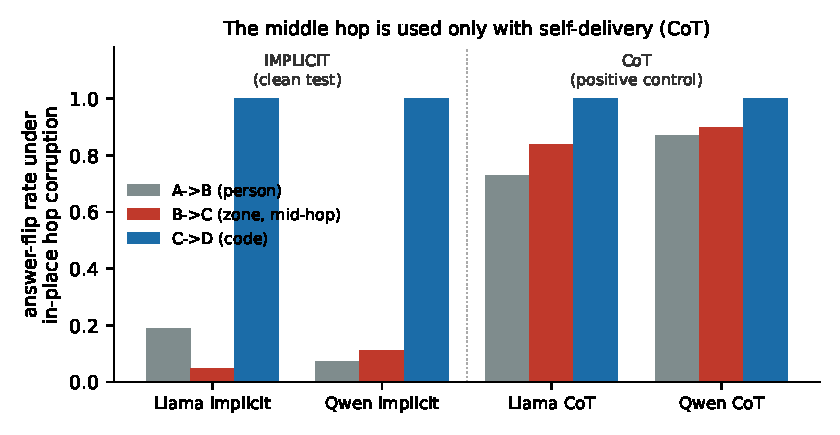
\includegraphics[width=0.82\textwidth]{figures/fig1_corruption.pdf}
\caption{The decisive panel. Corrupting the code fact ($C\!\to\!D$, blue) flips the
answer everywhere --- the code is read. But corrupting the middle hop ($B\!\to\!C$,
red) flips the implicit answer essentially never ($0.05$/$0.11$) while flipping the
CoT answer $0.84$/$0.90$. The same corruption machinery detects hop usage under CoT,
so the implicit null is a real null. The hop is used only when the model writes it
down.}
\label{fig:corr}
\end{figure}

\paragraph{(2) Mask-at-answer: only the code is consulted.}
Masking $A\!\to\!B$ or $B\!\to\!C$ at the answer-emitting step is inert (accuracy
$\approx$ full $\approx$ matched-filler control); masking $C\!\to\!D$ drives accuracy
to $0.000$ (Fig.~\ref{fig:gate2}). The answer step consults only the code fact: there
is no decode-time binding of the absent $D$ to disrupt.

\paragraph{(3) Decoy sweep: the elimination crutch is load-bearing.}
Removing the target's mid-hop still leaves the \emph{competitors'} facts, so the model
can deduce the target zone by elimination (``not in the other persons' zones''). Adding
decoy zones (a code fact with no person) makes the target indistinguishable once its
mid-hop is gone, blocking elimination. Under decoys, implicit accuracy floors to
chance (Llama $0.35\!\to\!0.07$, Qwen $0.45\!\to\!0.10$), while CoT stays flat
(Fig.~\ref{fig:decoy}). The flat CoT sweep is the critical control: identical decoys do
not hurt a model that actually traverses, so the implicit collapse is specifically the
loss of retrieval-and-elimination, not added distraction. Implicit success $\subset$
elimination.

\begin{figure}[t]
\centering
\begin{minipage}{0.49\textwidth}\centering
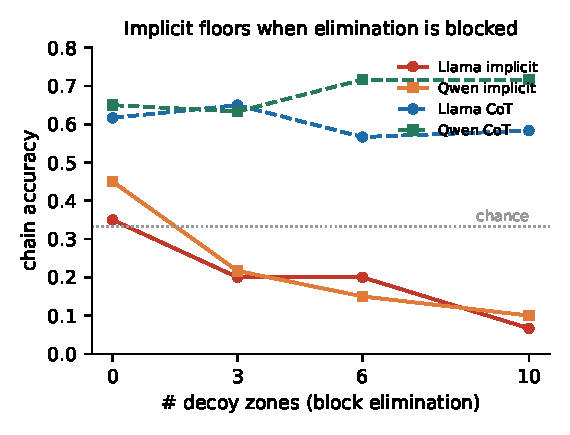
\includegraphics[width=\linewidth]{figures/fig2_decoy.pdf}
\caption{Decoy sweep. Blocking elimination floors implicit to chance (dotted) while
CoT is flat --- an orthogonal confirmation with its own control.}
\label{fig:decoy}
\end{minipage}\hfill
\begin{minipage}{0.49\textwidth}\centering
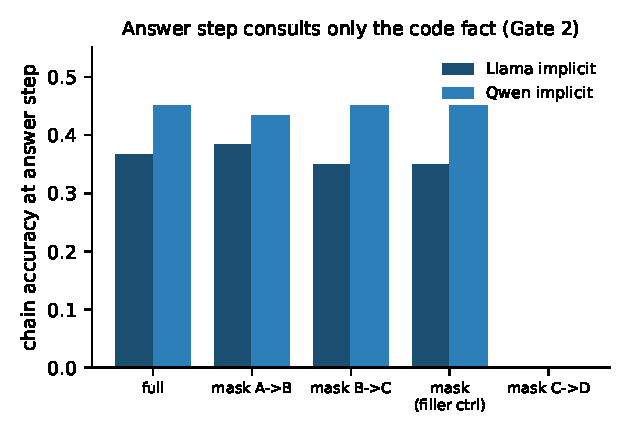
\includegraphics[width=\linewidth]{figures/fig3_gate2.pdf}
\caption{Gate 2 (implicit). Masking the link facts at the answer step is inert; only
masking the code fact kills the answer. No decode-time chain binding to disrupt.}
\label{fig:gate2}
\end{minipage}
\end{figure}

\subsection{Explicit CoT: genuine traversal, scaffolded by self-delivery}
\label{sec:cot}

With a written trace all three hops become causal (removal drop $+0.52$/$+0.57$ for the
mid-hop), corruption disrupts every hop, and the model follows a false mid-trail
$81\%$/$80\%$ of the time --- it genuinely routes through ``$B$ is in $C$''. It is
decoy-robust. But this is the pre-registered caveat: the model emits $B$, then $C$,
then $D$ as tokens, each delivered back into context and re-read. It composes by
\emph{externalizing} the hops (self-RAG), not by an internal decode-time binding.
Mask-at-answer is undefined for CoT (the answer token is many steps after the written
hops), so CoT sits outside the P1/P2/P3 trichotomy specific to the clean implicit test
and is reported as traversal-via-self-delivery. Its role here is twofold: a
demonstration that the corruption machinery \emph{can} detect traversal (the positive
control for \S\ref{sec:implicit}), and a mechanistic statement that the only way these
models traverse the chain is to write it down.

\subsection{A methodological catch: removal is confounded by elimination}
\label{sec:catch}

The pre-registration's literal Gate~0 (node \emph{removal}) under-states hop usage
under competition: a removed mid-fact is recoverable from the competitors, so removal
can read ``non-causal'' even for a used hop. The faithful test is in-place
\emph{corruption} (a false trail a traverser must follow), which cannot be
elimination-recovered. The removal$\leftrightarrow$corruption dissociation is itself
informative: Qwen-implicit's $A\!\to\!B$ is ``causal'' by removal ($-0.18$, it removes
the query anchor) yet inert under corruption (flip $0.07$) --- the model uses the
$A$-fact's \emph{presence} as a structural anchor, not the named entity. The critical
evidence mass for implicit success is essentially $\{C\!\to\!D\}$ alone.

\section{Discussion}
\label{sec:discuss}

\paragraph{The arc closes on one locus, three times.}
Attention redirection is transport~\cite{paper3retention}; stored-state correction is
not reusable and the repair is delivery of the binding~\cite{paper4arc}; and now
synthesis of an absent fact is, internally, retrieval-and-elimination, with real
composition appearing only when the steps are externalized. Three independent causal
gates, cross-model over two families and $1$B--$3$B, converge: \emph{this model class
delivers, and composes through an external buffer; it does not latently compute}. The
synthesis null is the strongest leg because synthesis is the one regime where a pure
transporter \emph{should} have failed --- the target is absent --- and the transport
reading still held.

\paragraph{Why this is a solid null, not a floor artifact.}
The implicit null is conditioned on baseline-\emph{correct} cases: even when the model
gets the chain right, it did so without using the middle hop. The same corruption test
detects usage under CoT ($0.84$--$0.90$), so the implicit $0.05$--$0.11$ is a real
null and not a broken probe. The decoy sweep adds an orthogonal manipulation with its
own flat-CoT control. Three operationalizations, a working positive control, and an
orthogonal manipulation all agree. As the pre-registration demanded, a positive after
a null streak warrants extra scrutiny --- and the one place a positive appeared (CoT)
is correctly attributed to self-delivery, not internal computation.

\paragraph{Product reading.}
Consistent with the program: for these model sizes do not expect latent multi-step
reasoning over delivered facts. Get composition by \emph{externalizing} it --- prompt
the model to write its steps (CoT), or run an explicit retrieve-compose-retrieve loop
(self-RAG / scratchpad) --- rather than hoping for an internal chain. ``Smarter'' on a
fixed model comes from the scaffold or from capacity, not from an internal shortcut.

\section{Limitations}
\label{sec:limits}

\begin{itemize}
\item \textbf{Regime.} Synthesis, \textbf{3B}, synthetic attr$\to$person$\to$zone$\to$code
chains, $N{=}4096$, $K{=}3$, greedy. A null is ``no decode-computation at 3B on this
design'', \emph{not} ``never''. Larger models, other chain types, and trained
composition are separate gates; the null does not transfer up.
\item \textbf{Low implicit baselines.} Implicit accuracy ($0.35$/$0.45$) is only
modestly above chance ($0.333$); the clean test sits near the floor edge. The verdict
is corruption-based and baseline-correct-conditioned, robust to the low baseline, but
a higher-headroom implicit chain would strengthen it.
\item \textbf{CoT is not internal computation.} CoT ``traversal'' is via self-delivery
(writing the steps); Gate~2 is undefined for it, so it is evidence of externalized
composition, not of decode-time binding.
\item \textbf{Open channel.} How implicit binds $A$ to the right code \emph{above
chance} without the named hops (some prefill-formed, elimination-assisted, structural
association) is left open --- it is not a traversal of the stated edges, but its exact
form is uncharacterized.
\item \textbf{Off-distribution interventions.} Mask-at-answer and corruption are
off-distribution; degeneration is expected and was required to be distinguished from
clean answer-death (specific wrong-endpoint), not miscounted.
\end{itemize}

\section{Conclusion}
\label{sec:conc}

At $3$B, implicit multi-hop synthesis of an absent fact does not occur: the model
retrieves a code and resolves the competition by elimination; corrupting the chain's
links leaves correct answers untouched, masking them at the answer step is inert, and
blocking elimination floors accuracy to chance. The model traverses the chain only
when permitted to \emph{write the steps}, converting computation into delivery. Across
attention, retrieval repair, and now synthesis --- three independent causal gates,
cross-model --- the finding is one: this model class transports and composes through
an external buffer; it does not latently compute. Internal decode-time composition,
if it exists, lives above $3$B or inside the scratchpad --- a separate gate.

\section*{Reproducibility}
The repository provides the pre-registration, the pilot/calibration and gate harnesses,
the raw per-case logs and per-cell gate aggregates for all four (model $\times$ mode)
cells, the chain-results stream, and the masking sanity gate; \texttt{make\_figures.py}
recomputes every figure from the gate aggregates. Llama-3.2-3B and Qwen2.5-3B; single
RTX~4060~Ti.

\begin{thebibliography}{99}
\small
\bibitem{paper3retention} E.\ Vyaltsev, D.\ Vyaltsev. \emph{No Critical Key Budget in Query-Axis Top-K Sparse Attention}. Zenodo, DOI 10.5281/zenodo.20514229, 2026.
\bibitem{paper4arc} E.\ Vyaltsev, D.\ Vyaltsev. \emph{The Bottleneck Is Delivery: Three Matched Controls Localize Long-Context Retrieval Failure}. Zenodo, 2026.
\bibitem{yang2024latent} S.\ Yang et al. \emph{Do Large Language Models Latently Perform Multi-Hop Reasoning?} ACL, 2024.
\bibitem{wang2024grokking} B.\ Wang et al. \emph{Grokked Transformers are Implicit Reasoners: A Mechanistic Journey to the Edge of Generalization}. NeurIPS, 2024.
\bibitem{wei2022cot} J.\ Wei et al. \emph{Chain-of-Thought Prompting Elicits Reasoning in Large Language Models}. NeurIPS, 2022.
\bibitem{lanham2023faithfulness} T.\ Lanham et al. \emph{Measuring Faithfulness in Chain-of-Thought Reasoning}. 2023.
\bibitem{balepur2024elimination} N.\ Balepur et al. \emph{Artifacts or Abduction: How Do LLMs Answer Multiple-Choice Questions Without the Question?} ACL, 2024.
\bibitem{matchedcontrols2026} E.\ Vyaltsev, D.\ Vyaltsev. \emph{Matched-Magnitude Controls for Mechanistic Claims in Attention}. Zenodo, DOI 10.5281/zenodo.20261207, 2026.
\end{thebibliography}

\end{document}
